
\documentclass[12pt]{article}
 
\usepackage[margin=1in]{geometry} 
\usepackage{amsmath,amsthm,amssymb}
\usepackage{pifont}
\usepackage{graphics}
\usepackage{graphicx}
\usepackage{array}
 
\newcommand{\N}{\mathbb{N}}
\newcommand{\Z}{\mathbb{Z}}
 
\newenvironment{theorem}[2][Theorem]{\begin{trivlist}
\item[\hskip \labelsep {\bfseries #1}\hskip \labelsep {\bfseries #2.}]}{\end{trivlist}}
\newenvironment{lemma}[2][Lemma]{\begin{trivlist}
\item[\hskip \labelsep {\bfseries #1}\hskip \labelsep {\bfseries #2.}]}{\end{trivlist}}
\newenvironment{exercise}[2][Exercise]{\begin{trivlist}
\item[\hskip \labelsep {\bfseries #1}\hskip \labelsep {\bfseries #2.}]}{\end{trivlist}}
\newenvironment{problem}[2][Problem]{\begin{trivlist}
\item[\hskip \labelsep {\bfseries #1}\hskip \labelsep {\bfseries #2.}]}{\end{trivlist}}
\newenvironment{question}[2][Question]{\begin{trivlist}
\item[\hskip \labelsep {\bfseries #1}\hskip \labelsep {\bfseries #2.}]}{\end{trivlist}}
\newenvironment{corollary}[2][Corollary]{\begin{trivlist}
\item[\hskip \labelsep {\bfseries #1}\hskip \labelsep {\bfseries #2.}]}{\end{trivlist}}

\newenvironment{solution}{\begin{proof}[Solution]}{\end{proof}}
 
\begin{document}
 
% --------------------------------------------------------------
%                         Start here
% --------------------------------------------------------------
 
\title{Homework 3}
\author{Georgios Kontoudis \textbullet{} gpkont@vt.edu\\ 
AOE5984 Cyber-Physical Systems \& Distributed Control\\
Professor Kyriakos Vamvoudakis} 
\date{Spring 2017}
 
\maketitle
\begin{exercise}{1} %theorem, exercise, problem, or question 
\textbf{Formation control with desired position offset using double integrator dynamics.}
\end{exercise}
\begin{solution}
For the double integrator dynamics
\begin{equation*}
\dot{x_i}=v_i\\
\end{equation*}
\begin{equation*}
\dot{v_i}=u_i, \hspace{.2cm} i=0,1, \hdots, N
\end{equation*}
where $x_i, v_i, u_i \in \mathbb{R}^2$ and the $0$ node is the leader agent.
The given formation control is 
\begin{equation*}
u_i= cK_p(\sum_{j\in N_i}a_{ij}(x_j-\Delta_j-x_i+\Delta_i)+g_i(x_0-x_i+\Delta_i))+
\end{equation*}
\begin{equation*}
+cK_d(\sum_{j\in N_i}a_{ij}(v_j-v_i)+g_i(x_0-x_i))
\end{equation*}
for a spanning tree, where $c>0$, $K_p=I_2$, $K_d=\gamma I_2$ and the leader has initial conditions and control $  x_0=\begin{bmatrix}
0\\
0
\end{bmatrix},  v_0=\begin{bmatrix}
1\\
1
\end{bmatrix}, u_o=\begin{bmatrix}
0\\
0
\end{bmatrix} $.

The spanning tree that we employed is depicted in figure \ref{graph}.
\begin{figure}[!h]
	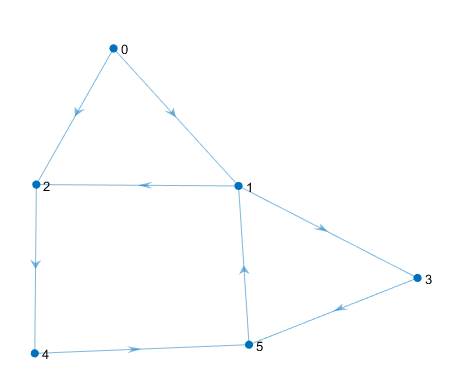
\includegraphics[scale=0.48]{figures/SpanningTree.png}
	\centering
	\caption{Spanning tree with 5 agents and a leader. The node $0$ is the leader.}
	\label{graph}
\end{figure}
\begin{figure}[!h]
	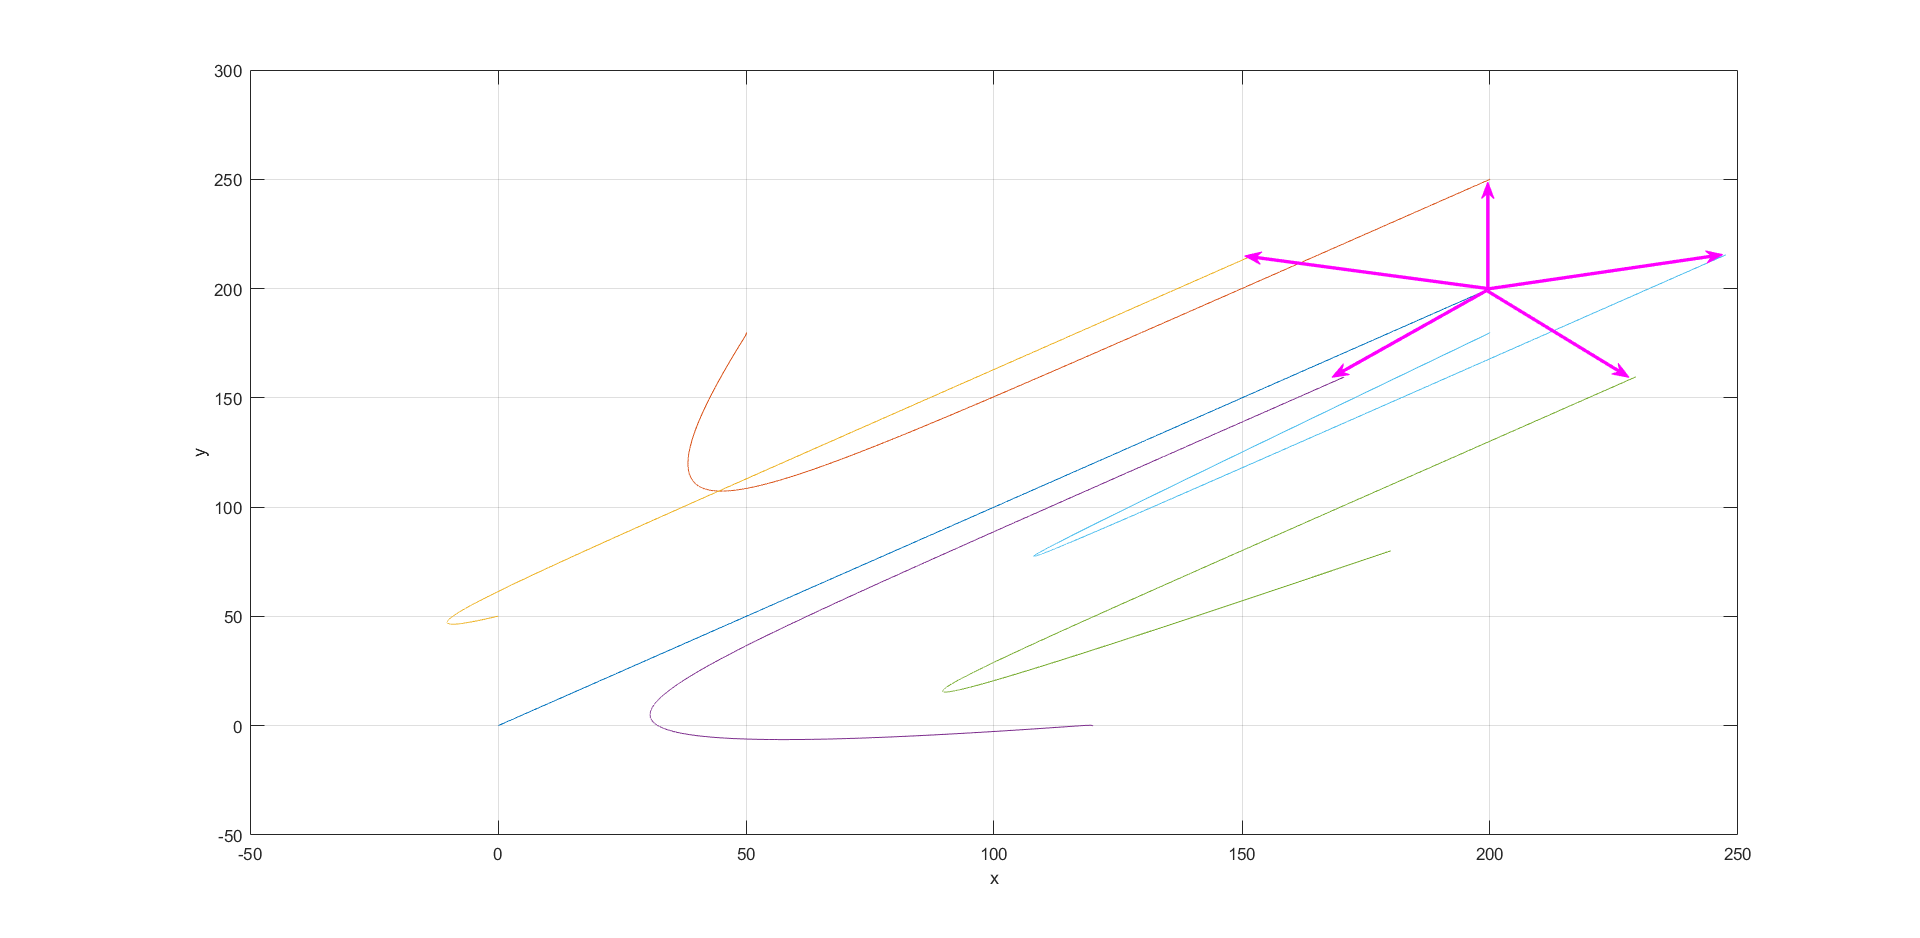
\includegraphics[scale=0.35]{figures/StarFormation.png}
	\centering
	\caption{Star formation of 6 agents.}
	\label{star_xy}
\end{figure}

The first formation of the agents was a star. The motion of the agents in the cartesian plane is presented in figure \ref{star_xy}. The initial positions were different for all agents, while the initial velocities were zero. Notice that the leader's motion followed a straight line, because its initial velocity was $v_x=1$, $v_y=1$.
\begin{figure}[!h]
	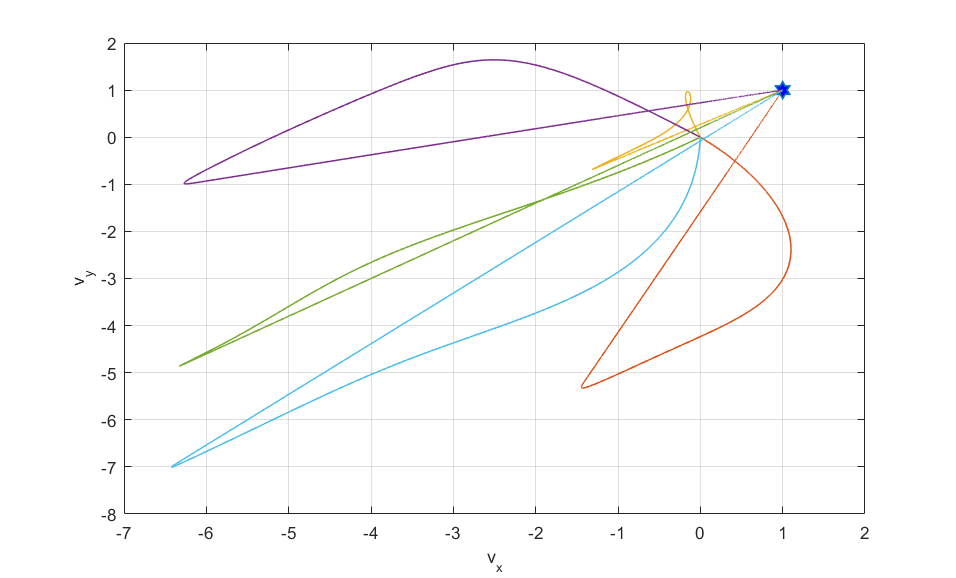
\includegraphics[scale=0.41]{figures/StarVelocities2D.png}
	\centering
	\caption{Agent velocities $v_x$, $v_y$ for star formation.}
	\label{starVel}
\end{figure}

An important aspect of the agent dynamics is the velocities. The velocities $v_x$, $v_y$ are shown in figure \ref{starVel}. All initial velocities of the agents were set to zero and they converged with the leader's velocity.  The agents velocities performance in time is presented in figure \ref{starVel_3D}. All agents converged with leader's velocity $v_x=1$, $v_y=1$.

\begin{figure}[!h]
	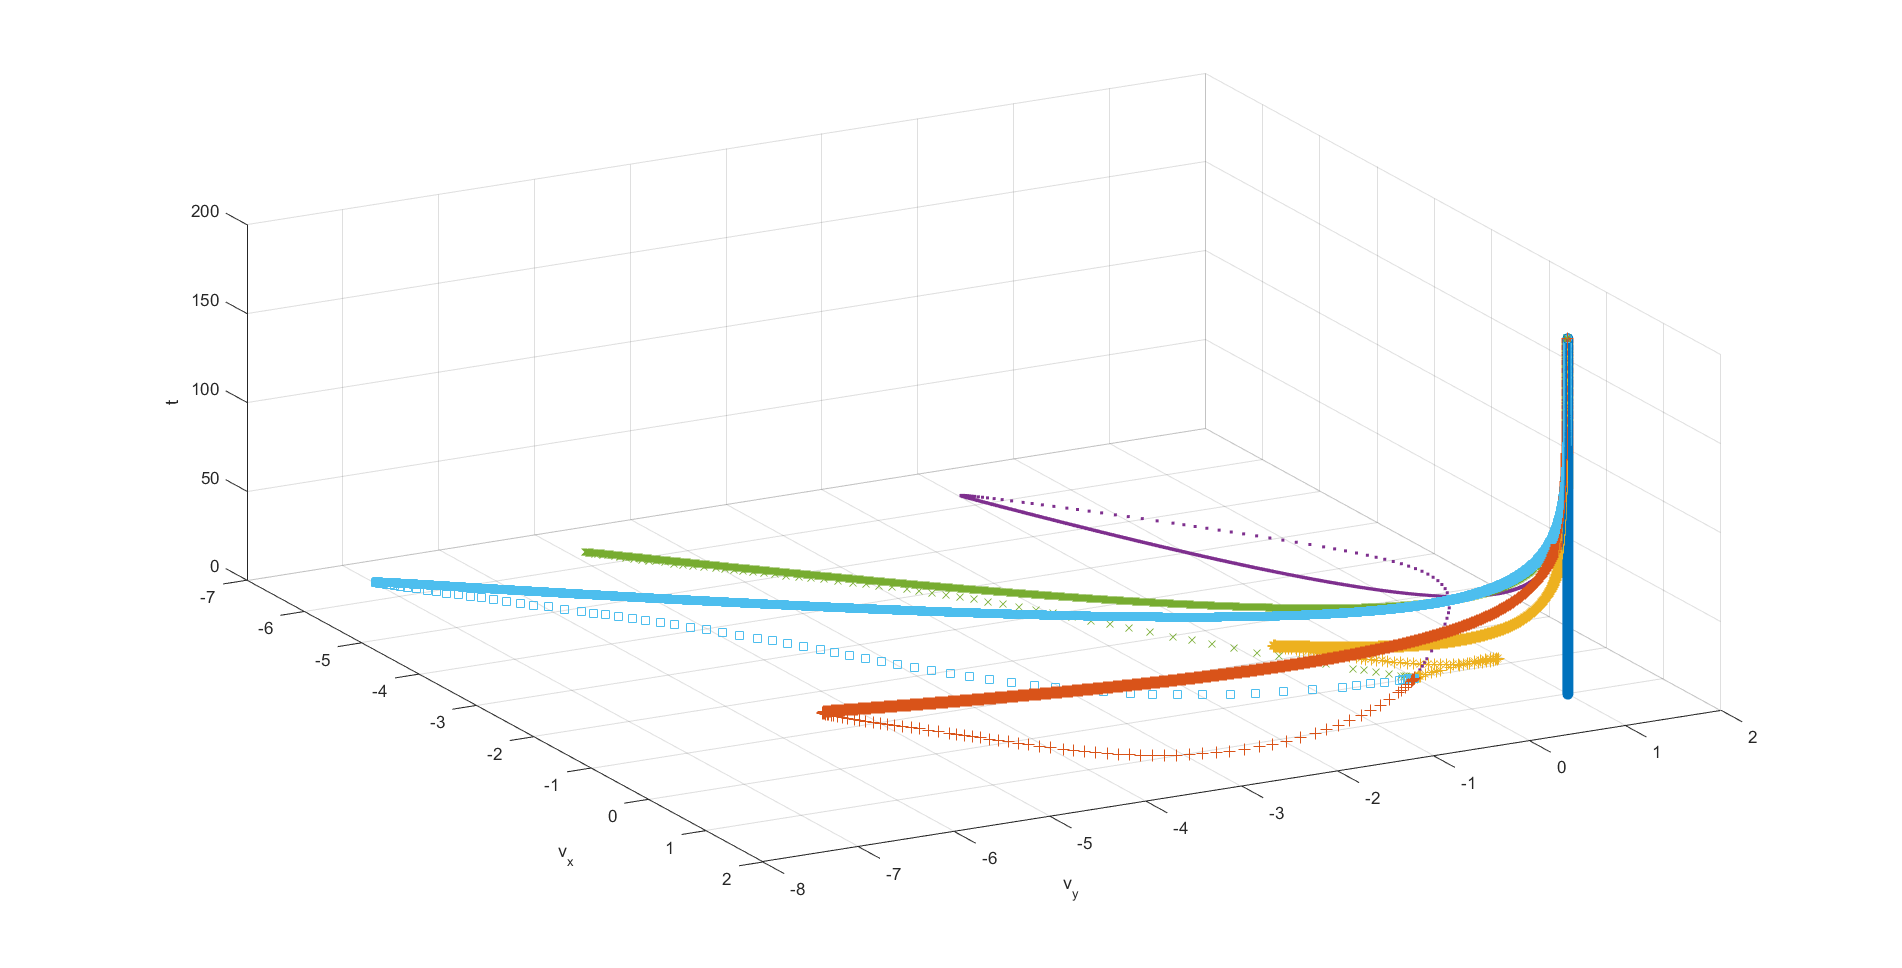
\includegraphics[scale=0.34]{figures/StarVelocities3D.png}
	\centering
	\caption{Agent velocities $v_x$, $v_y$ performance in time for star formation.}
	\label{starVel_3D}
\end{figure}
 
The next formation that we want to achieve is a polygon. Initial states remain as previously and the leader's final point in cartesian space is $(200,200)$. The polygon formation is depicted in figure \ref{polygon_xy}.  
\begin{figure}[!h]
	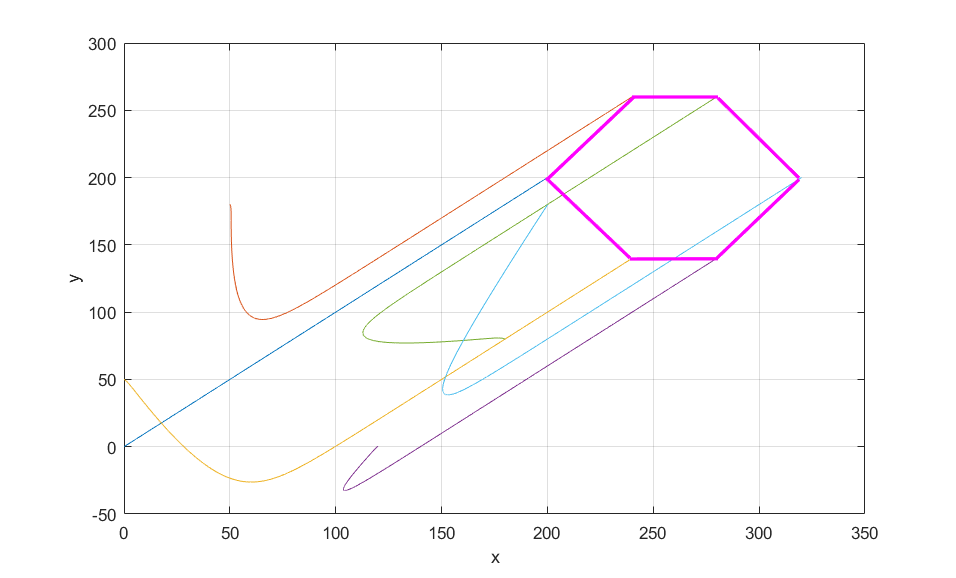
\includegraphics[scale=0.6]{figures/PolygonFormation.png}
	\centering
	\caption{Polygon formation of 6 agents.}
	\label{polygon_xy}
\end{figure}

\begin{figure}[!h]
	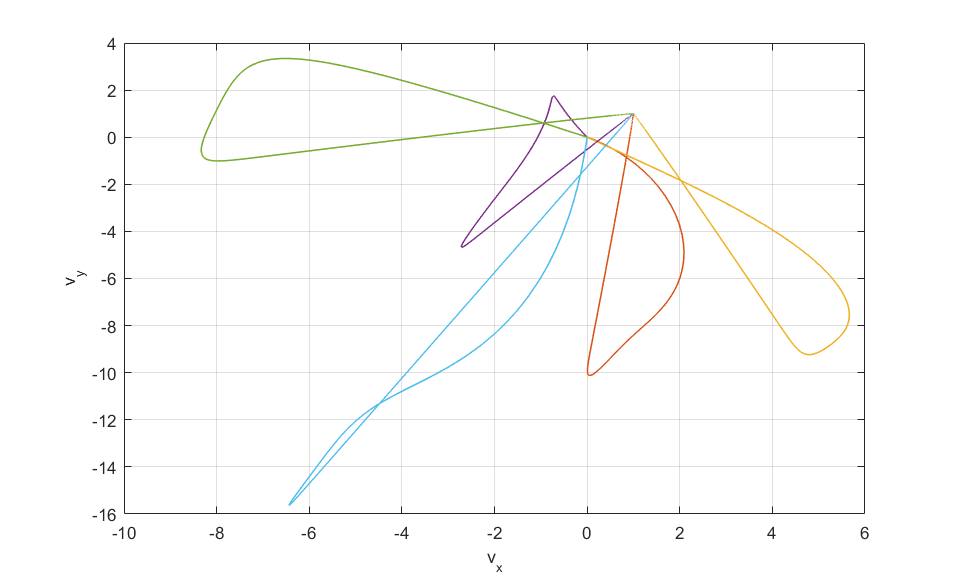
\includegraphics[scale=0.41]{figures/PolygonVelocities2D.png}
	\centering
	\caption{Agent velocities $v_x$, $v_y$ for polygon formation.}
	\label{polygonVel}
\end{figure}
\begin{figure}[!t]
	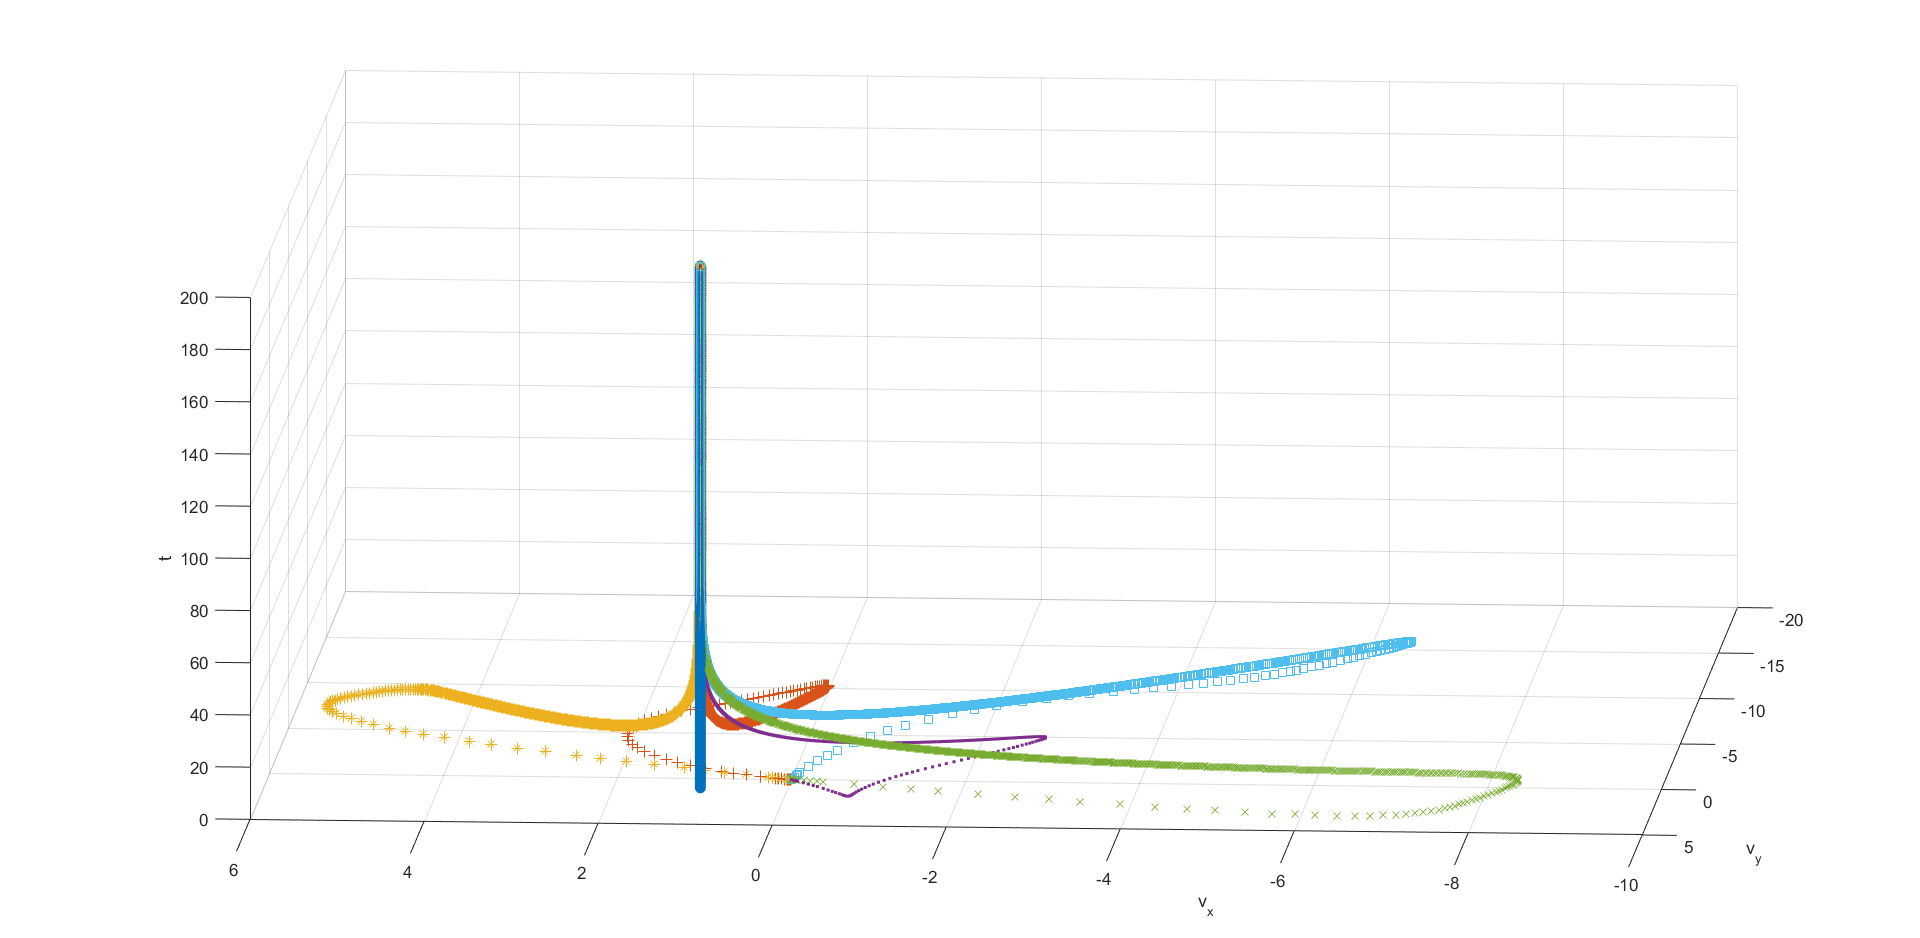
\includegraphics[scale=0.34]{figures/PolygonVelocities3D.png}
	\centering
	\caption{Agent velocities $v_x$, $v_y$ performance in time for polygon formation.}
	\label{polygonVel_3D}
\end{figure} 
Velocities of all agents converged with leader's initial velocity $v_x=1$, $v_y=1$ as presented in figure \ref{polygonVel}. Time performance of agent's velocities for polygon formation is shown in figure \ref{polygonVel_3D}.

The last formation that we want to achieve is a bracket. Initial states states remain as previously and the leader's final point in cartesian space is $(200,200)$. The bracket formation is depicted in figure \ref{bracket_xy}.  
\begin{figure}[!h]
	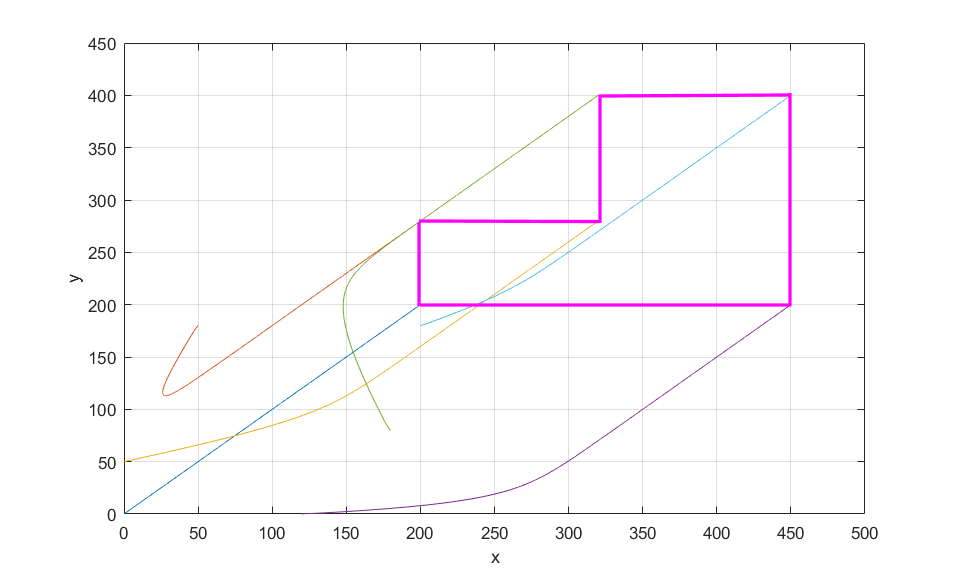
\includegraphics[scale=0.6]{figures/BracketFormation.png}
	\centering
	\caption{Bracket formation of 6 agents.}
	\label{bracket_xy}
\end{figure}

\begin{figure}[!h]
	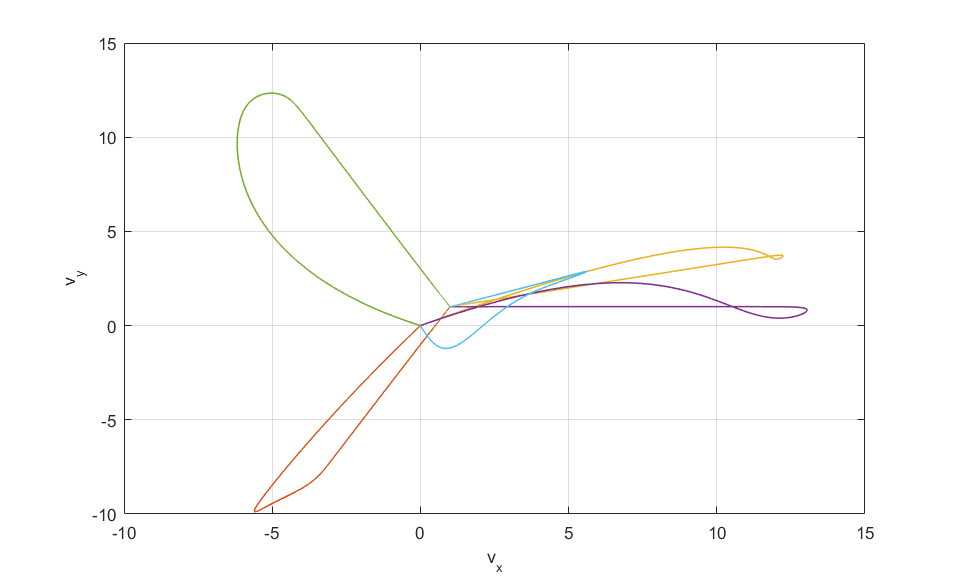
\includegraphics[scale=0.41]{figures/BracketVelocities2D.png}
	\centering
	\caption{Agent velocities $v_x$, $v_y$ for bracket formation.}
	\label{bracketVel}
\end{figure}
\begin{figure}[!t]
	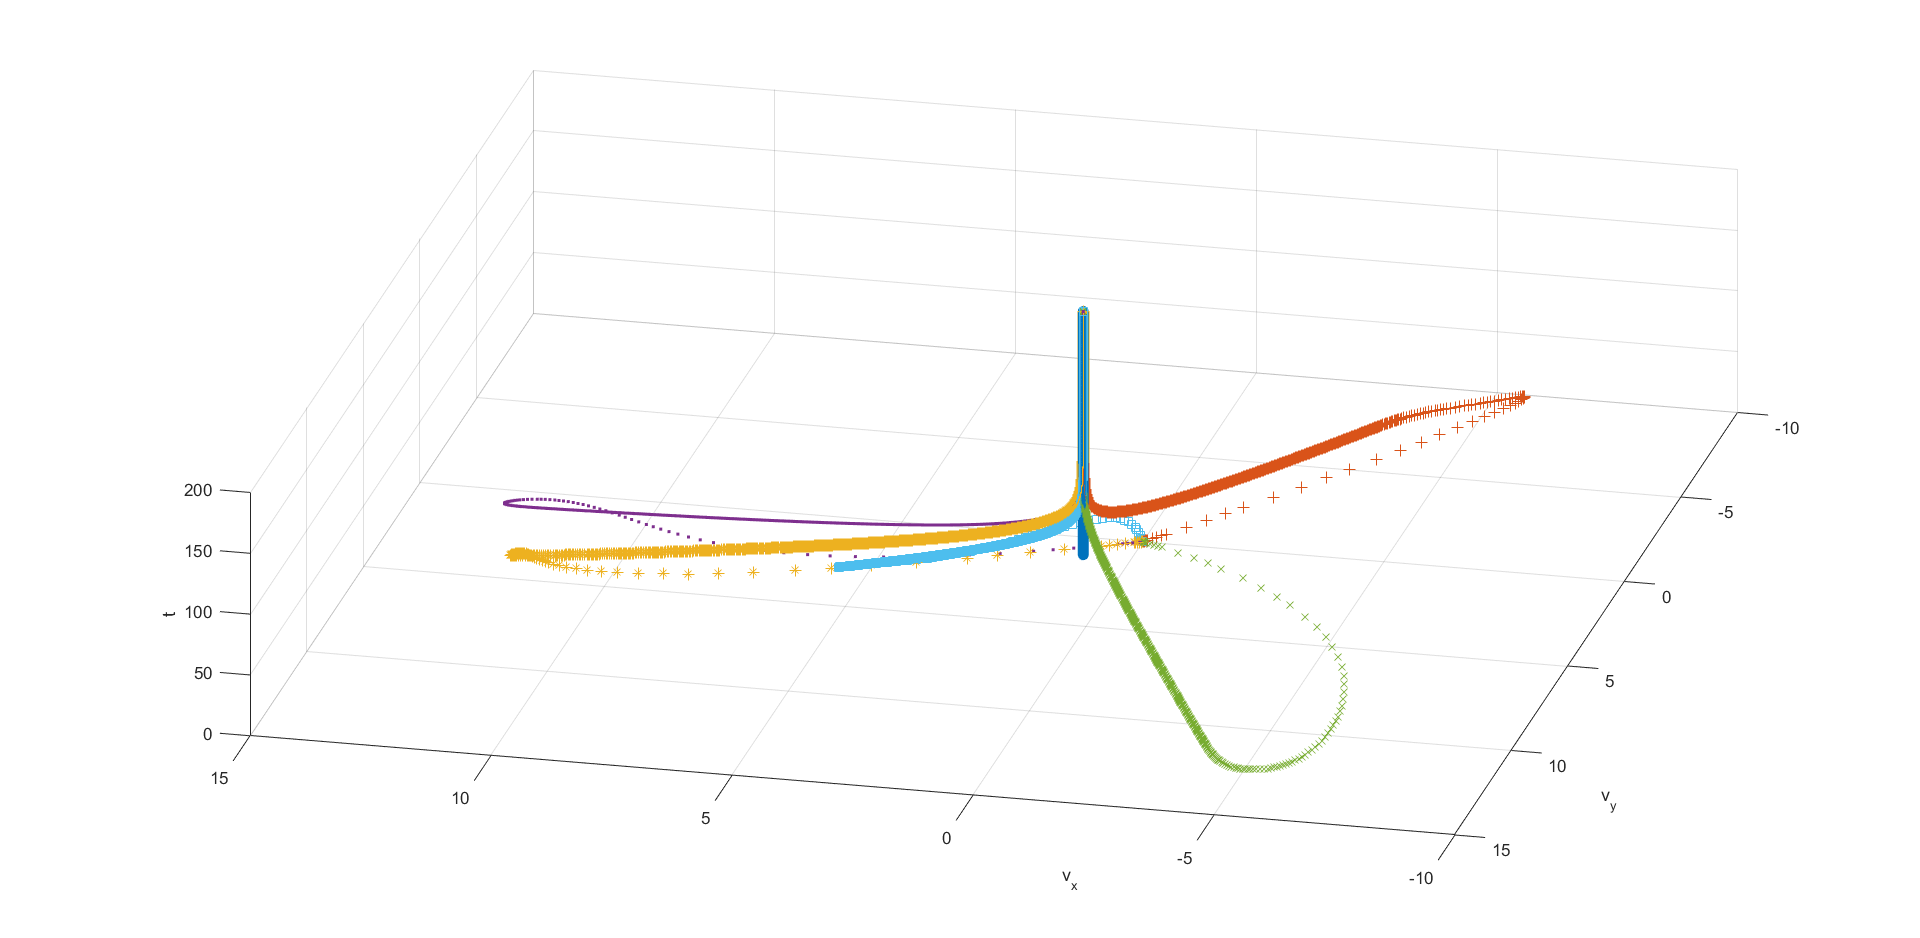
\includegraphics[scale=0.34]{figures/BracketVelocities3D.png}
	\centering
	\caption{Agent velocities $v_x$, $v_y$ performance in time for bracket formation.}
	\label{bracketVel_3D}
\end{figure} 
Velocities of all agents converged with leader's initial velocity $v_x=1$, $v_y=1$ as presented in figure \ref{bracketVel}. Time performance of agent's velocities for bracket formation is shown in figure \ref{bracketVel_3D}.

\end{solution}
\end{document}


